\documentclass[xcolor={dvipsnames}]{beamer}
%\usepackage[utf8]{inputenc}
%\usetheme{Madrid}
\usetheme{CambridgeUS}
\usecolortheme{}

%-------------------------------------------------------------------------------
%          -Packages nécessaires pour écrire en Français et en UTF8-
%-------------------------------------------------------------------------------
\usepackage[utf8]{inputenc}
\usepackage[french]{babel}
\usepackage[T1]{fontenc}
\usepackage{lmodern}
\usepackage{textcomp}

%-------------------------------------------------------------------------------

%-------------------------------------------------------------------------------
%                          -Outils de mise en forme-
%-------------------------------------------------------------------------------
\usepackage{hyperref}
\hypersetup{pdfstartview=XYZ}
\usepackage{enumerate}
\usepackage{graphicx}
%\usepackage{multicol}
%\usepackage{tabularx}

%\usepackage{anysize} %%pour pouvoir mettre les marges qu'on veut
%\marginsize{2.5cm}{2.5cm}{2.5cm}{2.5cm}

\usepackage{indentfirst} %%pour que les premier paragraphes soient aussi indentés
\usepackage{verbatim}
%\usepackage[table]{xcolor}  
%\usepackage{multirow}
\usepackage{ulem}
%-------------------------------------------------------------------------------


%-------------------------------------------------------------------------------
%                  -Nécessaires pour écrire des mathématiques-
%-------------------------------------------------------------------------------
\usepackage{amsfonts}
\usepackage{amssymb}
\usepackage{amsmath}
\usepackage{amsthm}
\usepackage{tikz}
\usepackage{xlop}
\usepackage[output-decimal-marker={,}]{siunitx}
%-------------------------------------------------------------------------------

%-------------------------------------------------------------------------------
%                  -Nécessaires pour écrire des formules chimiquess-
%-------------------------------------------------------------------------------

\usepackage[version=4]{mhchem}

%-------------------------------------------------------------------------------
%                    - Mise en forme 
%-------------------------------------------------------------------------------

\newcommand{\bu}[1]{\underline{\textbf{#1}}}


\usepackage{ifthen}


\newcommand{\ifTrue}[2]{\ifthenelse{\equal{#1}{true}}{#2}{$\qquad \qquad$}}

\newcommand{\kword}[1]{\textcolor{red}{\underline{#1}}}


%-------------------------------------------------------------------------------



%-------------------------------------------------------------------------------
%                    - Racourcis d'écriture -
%-------------------------------------------------------------------------------

% Angles orientés (couples de vecteurs)
\newcommand{\aopp}[2]{(\vec{#1}, \vec{#2})} %Les deuc vecteurs sont positifs
\newcommand{\aopn}[2]{(\vec{#1}, -\vec{#2})} %Le second vecteur est négatif
\newcommand{\aonp}[2]{(-\vec{#1}, \vec{#2})} %Le premier vecteur est négatif
\newcommand{\aonn}[2]{(-\vec{#1}, -\vec{#2})} %Les deux vecteurs sont négatifs

%Ensembles mathématiques
\newcommand{\naturels}{\mathbb{N}} %Nombres naturels
\newcommand{\relatifs}{\mathbb{Z}} %Nombres relatifs
\newcommand{\rationnels}{\mathbb{Q}} %Nombres rationnels
\newcommand{\reels}{\mathbb{R}} %Nombres réels
\newcommand{\complexes}{\mathbb{C}} %Nombres complexes


%Intégration des parenthèses aux cosinus
\newcommand{\cosP}[1]{\cos\left(#1\right)}
\newcommand{\sinP}[1]{\sin\left(#1\right)}

%Fractions
\newcommand{\myfrac}[2]{{\LARGE $\frac{#1}{#2}$}}

%Vocabulaire courrant
\newcommand{\cad}{c'est-à-dire}

%Droites
\newcommand{\dte}[1]{$(#1)$}
\newcommand{\fig}[1]{figure $#1$}
\newcommand{\sym}{symétrique}
\newcommand{\syms}{symétriques}
\newcommand{\asym}{axe de symétrie}
\newcommand{\asyms}{axes de symétrie}
\newcommand{\seg}[1]{$[#1]$}
\newcommand{\monAngle}[1]{$\widehat{#1}$}
\newcommand{\bissec}{bissectrice}
\newcommand{\mediat}{médiatrice}
\newcommand{\ddte}[1]{$[#1)$}

%Figures
\newcommand{\para}{parallélogramme}
\newcommand{\paras}{parallélogrammes}
\newcommand{\myquad}{quadrilatère}
\newcommand{\myquads}{quadrilatères}
\newcommand{\co}{côtés opposés}
\newcommand{\diag}{diagonale}
\newcommand{\diags}{diagonales}
\newcommand{\supp}{supplémentaires}
\newcommand{\car}{carré}
\newcommand{\cars}{carrés}
\newcommand{\rect}{rectangle}
\newcommand{\rects}{rectangles}
\newcommand{\los}{losange}
\newcommand{\loss}{losanges}


\newcommand{\homo}{homothétie}
\newcommand{\homos}{homothéties}




%----------------------------------------------------
% Environnements de cours
%------------------------------------------------------



%\usepackage{../../../../pas-math}
\usepackage{../../../moncours_beamer}





\graphicspath{{../img/}}
%Quelles sont les deux sortes de sources de lumière
\title{L'air qui nous entoure}
%\author{O. FINOT}\institute{Collège S$^t$ Bernard}


\AtBeginSection[]
{
	\begin{frame}
		\frametitle{}
		\tableofcontents[currentsection, hideallsubsections]
	\end{frame} 

}


\AtBeginSubsection[]
{
	\begin{frame}
		\frametitle{Sommaire}
		\tableofcontents[currentsection, currentsubsection]
	\end{frame} 
}

\begin{document}

\begin{frame}
  \titlepage 
\end{frame}

\section{Composition de l'air}



%
%\begin{frame}
%	\begin{alertblock}
%		\begin{itemize}
%			\item L'unité de mesure de l'\kw{intensité} électrique est l' \kw{ampère} (symbole $A$). 
%			
%			\item Un \kw{ampèremètre} permet de mesurer l'intensité du courant, il se branche \kw{en série} dans le circuit.
%		\end{itemize}
%			
%			
%		\begin{center}
%			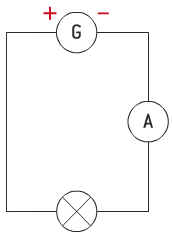
\includegraphics[scale=0.6]{img/schema1}
%		\end{center}
%	\end{alertblock}
%\end{frame}



\begin{frame}

\begin{mybilan}
	\begin{itemize}
		\item Un \kw{solide} a une \kw{forme propre} qui ne change pas, on peut le saisir.
		\item Un \kw{liquide} prend la \kw{forme du récipient} qui le contient.
		\item La surface d'un liquide en contact avec l'air est sa \kw{surface libre}.
		\item Au repos, cette surface libre est \kw{plane et horizontale}.
	\end{itemize}	   
\end{mybilan}
\end{frame}


\section{Pression et masse d'un gaz}

\subsection{Pression}

\begin{frame}

	\begin{mybilan}
	Pour décrire la vitesse d'un objet en mouvement, on utilise trois caractéristiques :
	\begin{itemize}
		\item la \kw{direction} (horizontale, verticale ou oblique), tangente à la trajectoire;
		
		\item le \kw{sens}, celui du mouvement (vers la gauche, vars la droite, vers le haut etc.);
		
		\item la \kw{valeur} exprimée m/s (ou km/h ou autre).
		
		Si le mouvement est uniforme, la relation \kw{$ v = \dfrac{d}{\Delta t} $}, permet de relier la vitesse de l'objet, la distance parcourue et la durée du parcours avec :
		\begin{itemize}
			\item d : distance parcourue en mètre (m)
			\item $\Delta t$ :durée du trajet en seconde (s)
			\item v : vitesse en mètre par seconde (m/s).
		\end{itemize}
	\end{itemize}



\end{mybilan}


\end{frame}


\subsection{Masse volumique}
\begin{frame}

	\begin{mybilan}
	
	\twoCol{
	\begin{center}
		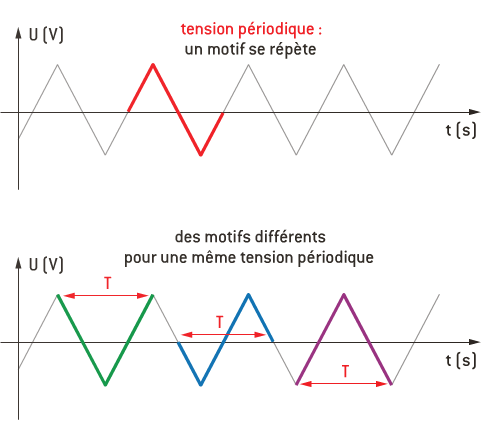
\includegraphics[scale=0.7]{bilan3}
	\end{center}

	\begin{itemize}
		\item Une tension est \kw{périodique} lorsque ses \kw{variations se répètent} identiques à elles mêmes au cours du temps. 
		\item La \kw{durée} d'un motif est la \kw{période}. On la note $T$, son unité est la seconde $s$.
	\end{itemize}
	}

\end{mybilan}
\end{frame}


%\section{Reconnaître le dioxyde de carbone}
%
%\begin{frame}
%	\begin{myact}{4 page 127}
	\begin{enumerate}
		\item Le gaz prélevé dans la seringue a été extrait d'eau pétillante par déplacement d'eau.\pause
		\item Au début de l'expérience, la solution d'eau de chaux est incolore et transparente.\pause
		\item Après y avoir fait barboter le gaz l'eau de chaux s'est troublée.\pause
		\item Un précipité blanc s'est formé lors de cette expérience, donc le gaz dissous dans l'eau pétillante est du dioxyde de carbone.
	\end{enumerate}
\end{myact}
%\end{frame}
%
%
%\begin{frame}
%	\begin{mybilan}
	\begin{itemize}
		\item La masse d'un corps est \kw{proportionnelle} à son volume; \pause
		\item Le coefficient de proportionnalité est la \kw{masse volumique} (notée $\rho$);\pause
		\item \kw{Un litre d'eau} a une masse de \kw{1 kilogramme};\pause
		\item Une substance est \kw{plus dense} qu'une autre si, pour un même volume, sa masse est supérieure.		
	\end{itemize}
\end{mybilan}
%\end{frame}

\end{document}